\section{Related Work}
\label{sec:related}

\begin{figure*}[t]
  \centering
%   \setlength{\abovecaptionskip}{0.cm}
  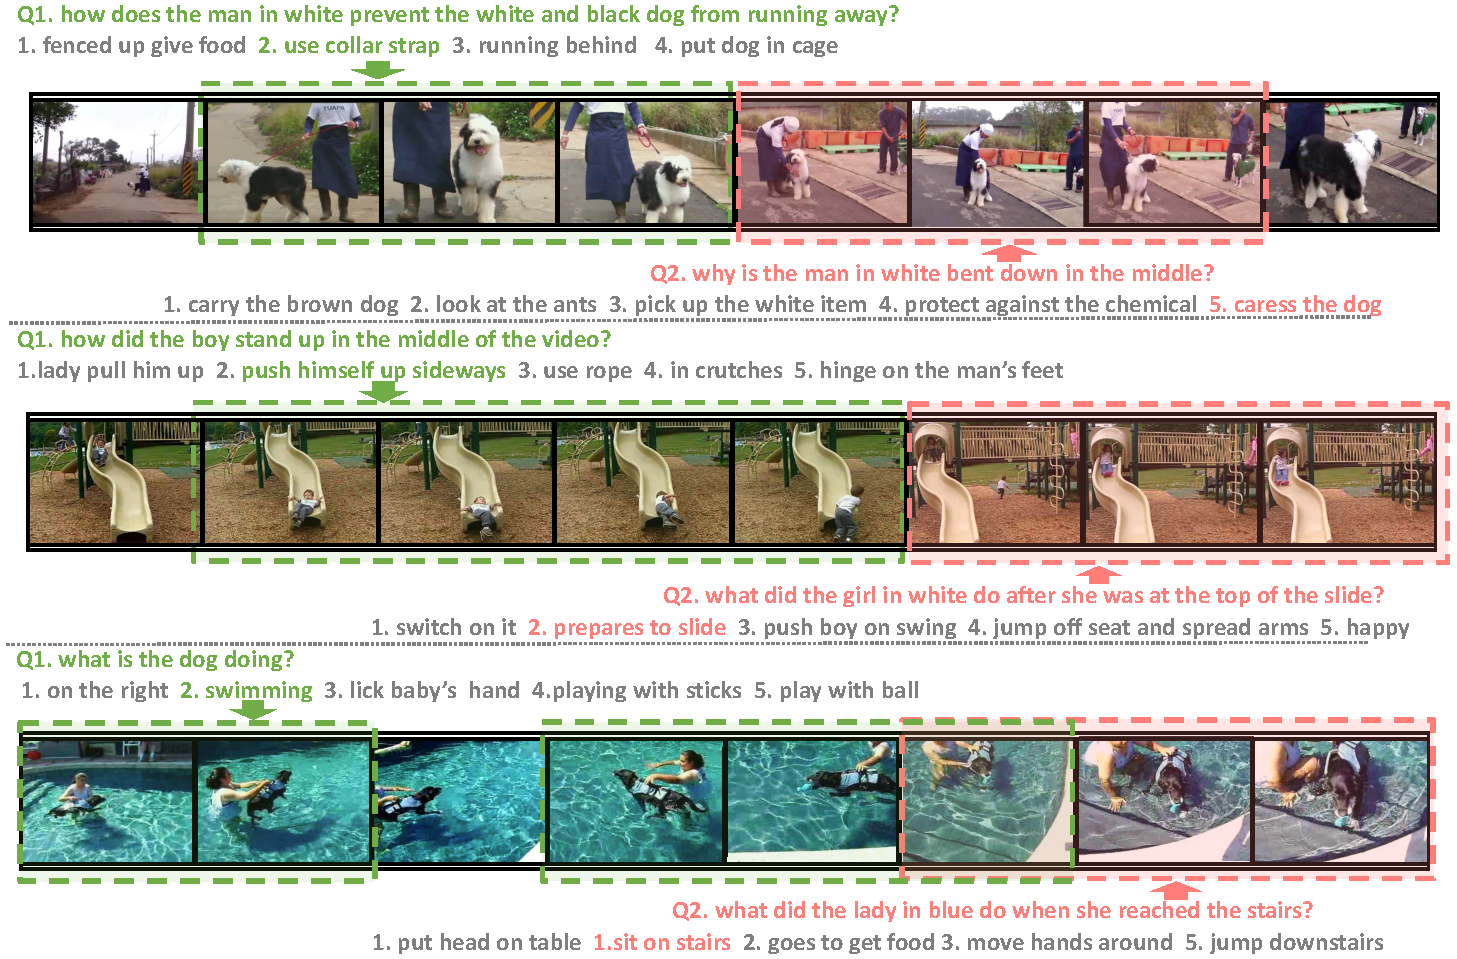
\includegraphics[width=0.97\textwidth]{fig/case.pdf}
 	\vspace{-13pt}
  \caption{Visualization of discovered grounding rationale. Each row comes with a video instance and two questions that target at different scene.  The \textcolor[rgb]{0,0.5,0}{green} and \textcolor[RGB]{225,152,150}{pink} windows indicate the rationales for the corresponding questions.}
  \label{fig:case-study}
 	\vspace{-10pt}
\end{figure*}

\vspace{5pt}
\noindent\textbf{Video Question Answering.}
Established to answer the question in dynamic visual content, VideoQA is bred through the task of ImageQA but has broadened its definition by assembling a temporal dimension. 
%
To make the task intriguing, the VideoQA benchmark has gone beyond the problem of description \cite{DBLP:conf/mm/XuZX0Z0Z17} and built several datasets to challenge temporal reasoning and even causal reflection \cite{DBLP:conf/cvpr/XiaoSYC21}. 
%
As a result, VideoQA has experienced an aggressive expansion in the architecture design. 
% 
Chronologically, early efforts tend to enact alignment through cross-modal attention \cite{zeng2016leveraging,li2019beyond} or enhanced memory design \cite{gao2018motionappearance, DBLP:conf/mm/XuZX0Z0Z17, fan2019heterogeneous}, while more recent works leverage the expressiveness of the graph neural network and perform the relation reasoning as node propagation \cite{jiang2020reasoning, DBLP:conf/mm/PengYBW21} or graph alignment \cite{park2021bridge}. 
%
In addition, current designs modify the representation of video and manipulate the temporal sequence from a hierarchical angle. Following this line, HCRN \cite{le2021hierarchical} first came out with the conditional relation module as building blocks that operate through different video intervals, whereas  HOSTR and PGAT made their advancement by incorporating visual content from different granularity. MSPAN, however, established cross-scale feature interaction on top of the hierarchy.
%
Despite effective, their intrinsic rationale has long been overlooked. To the best of our knowledge, EIGV is the first work that probes intrinsic interpretation. 

\vspace{5pt}
\noindent\textbf{Invariant Learning.}
% Given a encoder $f(\cdot)$ and input $x$, a representation $f(x)$ is equivariant to operation $G$, if $\forall x : f(G(x)) = T(G(x))$ ; Likewise, the property of invariance is defined as $\forall x : f(G(x)) = f(x)$. 
Given a encoder $f(\cdot)$ and input $x$, a representation $f(x)$ is invariant to operation $T$, if $\forall x : f(G(x)) = f(x)$. 
%
In practice, this invariant property has a long history in presenting visual content (\eg HOG \cite{DBLP:conf/mmm/HuangTHTJ11}), which has recently been renovated by deep learning in form of risk minimization. As its most prevailing form, IRM \cite{arjovsky2020invariant} fosters this philosophy by posing an environment invariant prior and discovering the underlying causal pattern by reducing cross-environment variance.   
% .that remains stable across different environments.
Different from previous studies that create environment via inductive re-grouping \cite{DBLP:conf/cvpr/AndersonWTB0S0G18} or adversarial inference \cite{DBLP:conf/icml/CreagerJZ21,wang2021causal, wang2022causal,wang2021clicks}, our method conducts causal intervention that perturbs the original sample distribution to form a new one.
\lyc{The most relvant work is \cite{Li_2022_CVPR}, where an invariant framework is introduced as a model-agnostic framework. However, EIGV gains better generalization ability by marrying equivariance as complementary learning principle.}
% Specifically, the discovery of  rationale implies two requirements on the partition:

\vspace{5pt}
\noindent\textbf{Visual Interpretability}
Machine interpretability can be achieved in various methods, such as clustering \cite{monnier2020dticlustering} or disentanglement \cite{shen2020interfacegan}. Our design can be vested in the category of attribution discovery, which investigates the contribution of different input elements toward the prediction. 
Based on whether the prediction and interpretation are yielded simultaneously, two categories are further defined: 1) post-hoc methods that generated the interpretation after prediction, such as backpropagation methods (\eg grad-CAM \cite{DBLP:conf/iccv/SelvarajuCDVPB17}). 2) self-interpretable method that cast prediction and interpretation at the same stage.
%
Unlike the post-hoc method that traces the interpretative clue from the output of the black-box, the self-interpretable model builds a transparency model via methods such as prototype generation \cite{DBLP:journals/corr/abs-1806-10574} or structural delineation \cite{wu2022dir}. 
%
In fact, previous works tend to focus on static image. EIGV, however, approaches the video interpretation in a multi-modal situation. 

\vspace{-5pt}